%
% resultat.tex 
%
% 
%
% !TEX root = ../../buch.tex
% !TEX encoding = UTF-8
%
%\usetikzlibrary{spy}
\section{Finale Überlegung\label{antennen:resultat}}

Das Kapitel \ref{antennen:ritzAnw} hat gezeigt, dass ein Abrundung an den Ecken
zur besten Effizienz führt, weil die abgerundete Form das Verhältnis \eqref{antennen:Verhältnis}
minimiert und somit die Effizienz maximiert. Wie gross der Radius dieser Abrundung
ist, muss jedoch noch bestimmt werden.


\subsection{Parametrisierung der abgerundeten Dreiecksantenne\label{antennen:param3eck}}
Die Länge $l$, hierbei der Umfang 
des abgerundeten Dreiecks, sowie dessen Fläche $A$ kann mit den Formeln
\definecolor{clrGreen}{RGB}{0, 117, 18}
\definecolor{drkOrange}{RGB}{255, 130, 28}
\begin{align}
	l &= \textcolor{blue}{2 \cdot \pi \cdot r} + \textcolor{drkOrange}{3 \cdot s - 6 \cdot \sqrt{3} \cdot r} \tag{20.24} \label{antennen:Länge} \\
	A &= \textcolor{clrGreen}{r^2 \cdot \pi} + \textcolor{black}{3 \cdot r \cdot (s - 2 \cdot \sqrt{3} \cdot r)} + \textcolor{darkred}{\frac{\sqrt{3} \cdot (s - 2 \cdot \sqrt{3} \cdot r)^2}{4}} \tag{20.25} \label{antennen:Fläche}
\end{align}\setcounter{equation}{25}%
berechnet werden.
Der Wirkungsgrad ist nun zu einem eindimensionalen Problem mit zwei Variablen geworden, das nur noch abhängig von 
der Seitenlänge $s$ des Dreiecks und des Radius $r$ der Kreise ist. Bildlich ist dies 
in Abbildung \ref{antennen:tikzdreieckAufteilung} veranschaulicht.
\begin{figure}
	\centering
	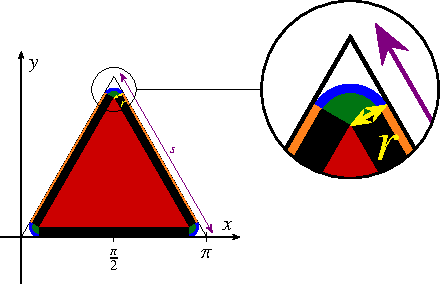
\includegraphics{papers/antennen/images/aufteilungDreieckZoom.pdf}
	\caption{Aufteilung des Dreiecks mit Zoom auf eine Ecke.}
	\label{antennen:tikzdreieckAufteilung}
\end{figure}

Durch Ableiten und Null setzten
\begin{equation}
	\frac{\partial}{\partial{r}} \bigg(\frac{l}{A^2}\bigg)=0
	\label{antennen:Ableitung}
\end{equation}
ergibt sich für eine gewünschte Seitenlänge $s$ ein Radius $r$ als Lösung. 
Die Ableitung ergibt die Gleichung 
\begin{equation}
	\frac{(- 4 \pi r + 12 \sqrt{3} r) (- 6 \sqrt{3} r + 2 \pi r + 3 s)}{\left(\pi r^{2} + 3 r (- 2 \sqrt{3} r + s) + \frac{\sqrt{3} \left(- 2 \sqrt{3} r + s\right)^{2}}{4}\right)^{3}} + \frac{- 6 \sqrt{3} + 2 \pi}{\left(\pi r^{2} + 3 r (- 2 \sqrt{3} r + s) + \frac{\sqrt{3} \left(- 2 \sqrt{3} r + s\right)^{2}}{4}\right)^{2}}=0.
	\label{antennen:Ableitunggelöst}
\end{equation}
Das Gleichungssystem ist äusserst hochgradig und komplex. Die Lösung erfolgt numerisch, 
wobei es eine Herausforderung darstellt, mögliche und unmögliche Ergebnisse voneinander zu unterscheiden.

Als konkretes Beispiel wird der Parameter $s$, also die Seitenlänge des Dreiecks mit dem Wert $\pi$ definiert. 
Nach dem Lösen der Gleichung \eqref{antennen:Ableitunggelöst} mit dem Python-Skript \cite{antennen:codeAbleitung} erhält
man den Wert $r\approx0.2465$. Das Verhältnis zwischen Seitenlänge und Radius ist somit $\frac{\pi}{0.2465} \approx 12.744$.
Dieses Verhältnis kann nun für beliebige Seitenlängen verwendet werden und stellt somit eine wertvolle Hilfe für 
diejenigen dar, die eine optimale dreieckige Loop-Antenne entwerfen möchten.

\subsection{Fazit\label{antennen:fazit}}
In diesem Kapitel wurde eine dreieckige Antennenform ermittelt, welche die optimale Effizienz aufweist. Mittels dem Variationsprinzip von Ritz wurde dargelegt, dass eine Antenne in Form eines gleichseitigen Dreiecks für eine Effizienzsteigerung abgerundete Ecken benötigt. Das Verhältnis zwischen Seitenlänge und Radius $\frac{\pi}{0.2465} \approx 12.744$ ist optimal.
